\documentclass[t, 9pt,xcolor=dvipsnames]{beamer}

%Insert number of slides
\beamertemplatenavigationsymbolsempty
\addtobeamertemplate{navigation symbols}{}{%
    \usebeamerfont{footline}%
    \usebeamercolor[fg]{footline}%
    \hspace{1em}%
    \insertframenumber/\inserttotalframenumber
}

%Define colors useful for presentation
\definecolor{UniBlue}{RGB}{0,102,204}
\definecolor{UniOrange}{RGB}{255,128,0}
\definecolor{mygreen}{RGB}{120,190,33}
\newcommand{\green}[1]{\textcolor{ForestGreen}{#1}}

\setbeamercolor{title}{fg=UniBlue}
\setbeamercolor{frametitle}{fg=UniBlue}
\setbeamercolor{structure}{fg=UniBlue}
\setbeamercolor{footline}{fg=black}
\setbeamercolor{caption name}{fg=black}
\setbeamercolor{bibliography item}{fg=black}
\setbeamercolor*{bibliography entry title}{fg=black}
\setbeamercolor*{bibliography entry author}{fg=black}
\setbeamercolor*{bibliography entry location}{fg=black}
\setbeamercolor*{bibliography entry note}{fg=black}

\setbeamertemplate{section in toc}[sections numbered]
\setbeamertemplate{caption}[numbered]
\setbeamertemplate{bibliography item}{\insertbiblabel}

%Additional packages
\usepackage{blkarray}
\usepackage{amsmath}
\usepackage{amsfonts}
\usepackage{amssymb}
\usepackage{algorithm2e}
\usepackage{appendixnumberbeamer}
\usepackage{pgfplots}
\usepgfplotslibrary{groupplots,dateplot}
\usetikzlibrary{patterns,shapes.arrows}
\pgfplotsset{compat=newest}
\usepackage{multimedia}
\usepackage{media9}
\usepackage{pbox}
\usepackage{multirow}
\usepackage[makeroom]{cancel}
\usepackage[export]{adjustbox}
\usepackage{tabularx}
\usepackage{caption}
\usepackage{xcolor}
\usepackage{tikz,pgfplotstable,filecontents}
\usepackage{listings}
\usepackage{enumitem}


%Shading text: useful to highlight information
\usepackage{framed, color}
\definecolor{shadecolor}{RGB}{220,220,220}
\usepackage{makecell}

%New commands
\newcommand{\code}[1]{{\fontfamily{pcr}\selectfont #1}}
\renewcommand{\vec}[1]{\boldsymbol{#1}}         % for vectors
\newcommand{\mat}[1]{\boldsymbol{#1}}           % for matrices
\newcommand{\pp}[1]{\left(#1\right)}
\newcommand{\dd}[2]{\frac{\partial #1}{\partial #2}}
\newcommand{\grad}{\nabla}
% \captionsetup[algorithm]{labelformat=empty}

\usepackage{subcaption}
%Define logos for subojectives
% \newcommand{\logoso1}{\setbeamertemplate{logo}{\includegraphics[width=0.1\textwidth]{images/so1.png}}
\def\mathunderline#1#2{\color{#1}\underline{{\color{black}#2}}\color{black}}


\usepackage{siunitx}

\lstnewenvironment{PYTHON}
{
	\lstset{frame=tb,
		language=python,
		aboveskip=3mm,
		belowskip=3mm,
		showstringspaces=false,
		columns=flexible,
		basicstyle={\small\ttfamily},
		numbers=none,
		numberstyle=\tiny\color{gray},
		keywordstyle=\color{blue},
		commentstyle=\color{green},
		stringstyle=\color{purple},
		breaklines=true,
		breakatwhitespace=true,
		tabsize=3}
}
{}


% Add an outline slide at the beginning of each new section
\AtBeginSection[]
{
	{
		\setbeamertemplate{footline}{} %this line removes slides numbers
		\begin{frame}[noframenumbering]
			\frametitle{Outline}
			\tableofcontents[currentsection]
		\end{frame}
	}
}

\title{\textbf{Understanding iterative linear solvers for sparse systems}}
\subtitle{Group meeting}
\author{Bruno Blais}


\begin{document}
    %% Title slide
	\begin{frame}
	\vspace{0.5cm}
		\begin{figure}
	  		
\includegraphics[scale = 0.12]{images/logo_lethe.png}\hspace*{0.2cm}
	  		
\includegraphics[scale = 0.4]{images/logo-poly.jpg}
		\end{figure}
		\titlepage
	\end{frame}
	
	%%Contents slide
	\begin{frame}
		\frametitle{\textbf{Outline}}
		\tableofcontents
	\end{frame}
	
	%% Other slides
	\section{Context and motivation}
	\begin{frame}
	\frametitle{\textbf{1. Context and motivation}}

    \visible<1->{
    \begin{shaded}
    \textbf{Why?}
    \begin{itemize}
        \item Linear solvers play a large role in the Lethe workflow for FEM simulations.
        \item Hard to self-study.
    \end{itemize}
    \end{shaded}}

    \visible<2->{
    \begin{shaded}
    \textbf{What is covered?}
    \begin{itemize}
        \item Establish two canonical problems which lead to sparse linear systems.
        \item Present four iterative solvers in order of complexity:
        \begin{itemize}
        	\item Jacobi (very easy)
        	\item Gauss Seidel (easy)
        	\item Conjugate Gradient (hard)
        	\item GMRES (very hard)
        \end{itemize}
    \end{itemize}
    \end{shaded}}
    % \vspace{0.4cm}
    \visible<3->{
	\begin{shaded}
		\textbf{What is \textbf{not} covered?}
		\begin{itemize}
			\item Preconditioning
			\item Sparse data structure for matrices
		\end{itemize}
		\end{shaded}}

\end{frame}
	
	\section{Problems}
	\begin{frame}
	\frametitle{\textbf{1. Problem A: Steady-state Poisson equation}}
    
    Consider a $2$-dimensional unit square $\Omega = (0,1)^d$ and the following problem subjected to homogeneous Dirichlet boundary conditions: 
    \vspace{0.5cm}
    \begin{columns}[c]
    \begin{column}{0.5\textwidth}
    % \vspace*{-\baselineskip}
    \begin{framed}
    Find a scalar $T$ in $\Omega \rightarrow \mathbb{R}$ satisfying:
    \begin{align*}
        -\partial_j \partial_j T =& 10 \ \textrm{ in } \Omega\\
         T =& 0 \ \textrm{ in } \Gamma
    \end{align*}
    \end{framed}
    \end{column}
    \begin{column}{0.4\textwidth}
    \vspace*{-\baselineskip}
    \begin{center}
    	
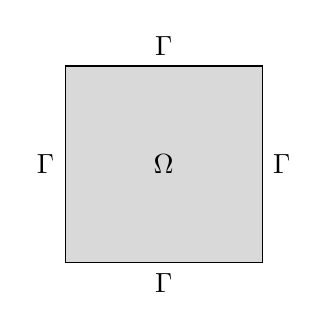
\begin{tikzpicture}[scale=2.5]
	% Draw the shaded square
	\fill[gray!30] (0,0) rectangle (1,1);
	
	% Draw the square outline
	\draw (0,0) rectangle (1,1);
	
	% Label Ω inside the square
	\node at (0.5,0.5) {$\Omega$};
	
	% Label Γ on the boundaries
	\node at (-0.1,0.5) {$\Gamma$};
	\node at (1.1,0.5) {$\Gamma$};
	\node at (0.5,-0.1) {$\Gamma$};
	\node at (0.5,1.1) {$\Gamma$};
\end{tikzpicture}
	   %\includegraphics[scale = 0.13]{images/domain.png}
	   %\includegraphics[scale = 0.13]{images/domain_3d.png}
    \end{center}
    \end{column}
    \end{columns}
    
    \vspace{0.4cm}
    \begin{itemize}
        \item This is a Poisson problem for $T$. 
    \end{itemize}    

\end{frame}


\begin{frame}
\frametitle{\textbf{1. Problem B: Steady-state Advection-diffusion equation}}

Consider a $2$-dimensional unit square $\Omega = (0,1)^d$ and the following problem subjected to homogeneous Dirichlet boundary conditions: 
\vspace{0.5cm}
\begin{columns}[c]
	\begin{column}{0.5\textwidth}
		% \vspace*{-\baselineskip}
		\begin{framed}
			Find a scalar $T$ in $\Omega \rightarrow \mathbb{R}$ satisfying:
			\begin{align*}
				u_j \partial_j T - \epsilon \partial_j \partial_j T =& 10\ \textrm{ in } \Omega\\
				T =& 0 \ \textrm{ in } \Gamma \\
				u_j =& 1 \ \forall j \in [1,d]
			\end{align*}
		\end{framed}
	\end{column}
	\begin{column}{0.4\textwidth}
		\vspace*{-\baselineskip}
		\begin{center}
			
			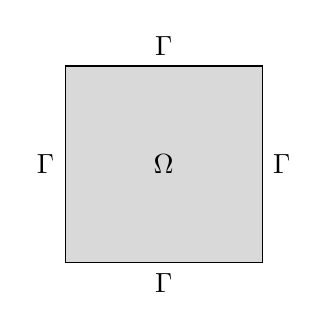
\begin{tikzpicture}[scale=2.5]
				% Draw the shaded square
				\fill[gray!30] (0,0) rectangle (1,1);
				
				% Draw the square outline
				\draw (0,0) rectangle (1,1);
				
				% Label Ω inside the square
				\node at (0.5,0.5) {$\Omega$};
				
				% Label Γ on the boundaries
				\node at (-0.1,0.5) {$\Gamma$};
				\node at (1.1,0.5) {$\Gamma$};
				\node at (0.5,-0.1) {$\Gamma$};
				\node at (0.5,1.1) {$\Gamma$};
			\end{tikzpicture}
			%\includegraphics[scale = 0.13]{images/domain.png}
			%\includegraphics[scale = 0.13]{images/domain_3d.png}
		\end{center}
	\end{column}
\end{columns}

\vspace{0.4cm}
\begin{itemize}
	\item This is an Advection-Diffusion problem for $T$. 
	\item The value of $\frac{1}{\epsilon}$ controls the Péclet number ($\mathrm{Pe}=\frac{1}{\epsilon}$).
	\item The higher the Péclet number is, the more hyperbolic the equation becomes.
\end{itemize}    

\visible<2->{
	\textcolor{UniBlue}{$\longrightarrow$ The next step is to discretize the equation using the \textbf{finite difference method}.}}
\end{frame}


\begin{frame}
	\frametitle{\textbf{1. Problem A: FDM}}
	
	\begin{columns}[c]
		\begin{column}{0.5\textwidth}
			% \vspace*{-\baselineskip}
			\begin{framed}
				Find a scalar $T$ in $\Omega \rightarrow \mathbb{R}$ satisfying:
				\begin{align*}
					\partial_j \partial_j T =& 1 \ \textrm{ in } \Omega\\
					T =& 0 \ \textrm{ in } \Gamma
				\end{align*}
			\end{framed}
		\end{column}
		\begin{column}{0.4\textwidth}
			\vspace*{-\baselineskip}
			\begin{center}
				
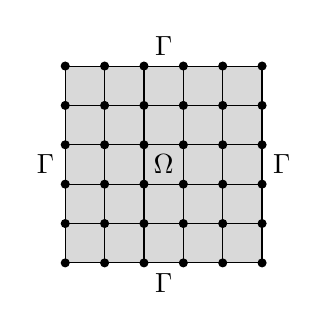
\begin{tikzpicture}[scale=2.5]
	% Draw the square outline
\fill[gray!30] (0,0) rectangle (1,1);
	
    
% Draw the grid lines inside the square
\foreach \x in {0.2,0.4,0.6,0.8}
\draw (\x,0) -- (\x,1);
\foreach \y in {0.2,0.4,0.6,0.8}
\draw (0,\y) -- (1,\y);

% Draw the grid lines outside the square
\draw (0,0) grid (1,1);

% Draw circles inside the square and in the corners
\foreach \x in {0.2,0.4,0.6,0.8}
\foreach \y in {0.2,0.4,0.6,0.8}
\filldraw (\x,\y) circle (0.02);
\foreach \x in {0,1}
\foreach \y in {0,1}
\filldraw (\x,\y) circle (0.02);

% Label Ω inside the square
\node at (0.5,0.5) {$\Omega$};

% Label Γ on the boundaries
\node at (-0.1,0.5) {$\Gamma$};
\node at (1.1,0.5) {$\Gamma$};
\node at (0.5,-0.1) {$\Gamma$};
\node at (0.5,1.1) {$\Gamma$};

% Draw nodes on the sides
\foreach \x in {0.2,0.4,0.6,0.8}
\filldraw (\x,0) circle (0.02);
\foreach \y in {0.2,0.4,0.6,0.8}
\filldraw (0,\y) circle (0.02);
\foreach \x in {0.2,0.4,0.6,0.8}
\filldraw (\x,1) circle (0.02);
\foreach \y in {0.2,0.4,0.6,0.8}
\filldraw (1,\y) circle (0.02);

\end{tikzpicture}
				%\includegraphics[scale = 0.13]{images/domain.png}
				%\includegraphics[scale = 0.13]{images/domain_3d.png}
			\end{center}
		\end{column}
	\end{columns}
	
	\vspace{0.4cm}
We divide the domain into a grid and obtain:
\begin{align*}
	\frac{1}{\Delta x^2} \pp{-T_{i+1} + 2T_{i} - T_{i-1}} + \frac{1}{\Delta y^2} \pp{-T_{i+n_x} + 2T_{i} - T_{i-n_x}} &= 1  \ \forall i \in \Omega
	\\
	T_i &= 0 \  \forall i \in \Gamma
\end{align*}  
\end{frame}

\begin{frame}
	\frametitle{\textbf{1. Problem B: FDM}}
	
	\begin{columns}[c]
		\begin{column}{0.5\textwidth}
			% \vspace*{-\baselineskip}
		\begin{framed}
	Find a scalar $T$ in $\Omega \rightarrow \mathbb{R}$ satisfying:
	\begin{align*}
		u_j \partial_j T + \epsilon \partial_j \partial_j T =& 1 \ \textrm{ in } \Omega\\
		T =& 0 \ \textrm{ in } \Gamma \\
		u_j =& 1 \ \forall j \in [1,d]
	\end{align*}
\end{framed}
		\end{column}
		\begin{column}{0.4\textwidth}
			\vspace*{-\baselineskip}
			\begin{center}
				
				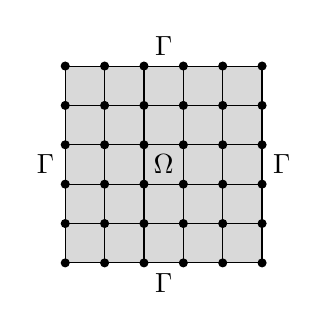
\begin{tikzpicture}[scale=2.5]
					% Draw the square outline
					\fill[gray!30] (0,0) rectangle (1,1);
					
					
					% Draw the grid lines inside the square
					\foreach \x in {0.2,0.4,0.6,0.8}
					\draw (\x,0) -- (\x,1);
					\foreach \y in {0.2,0.4,0.6,0.8}
					\draw (0,\y) -- (1,\y);
					
					% Draw the grid lines outside the square
					\draw (0,0) grid (1,1);
					
					% Draw circles inside the square and in the corners
					\foreach \x in {0.2,0.4,0.6,0.8}
					\foreach \y in {0.2,0.4,0.6,0.8}
					\filldraw (\x,\y) circle (0.02);
					\foreach \x in {0,1}
					\foreach \y in {0,1}
					\filldraw (\x,\y) circle (0.02);
					
					% Label Ω inside the square
					\node at (0.5,0.5) {$\Omega$};
					
					% Label Γ on the boundaries
					\node at (-0.1,0.5) {$\Gamma$};
					\node at (1.1,0.5) {$\Gamma$};
					\node at (0.5,-0.1) {$\Gamma$};
					\node at (0.5,1.1) {$\Gamma$};
					
					% Draw nodes on the sides
					\foreach \x in {0.2,0.4,0.6,0.8}
					\filldraw (\x,0) circle (0.02);
					\foreach \y in {0.2,0.4,0.6,0.8}
					\filldraw (0,\y) circle (0.02);
					\foreach \x in {0.2,0.4,0.6,0.8}
					\filldraw (\x,1) circle (0.02);
					\foreach \y in {0.2,0.4,0.6,0.8}
					\filldraw (1,\y) circle (0.02);
					
				\end{tikzpicture}
				%\includegraphics[scale = 0.13]{images/domain.png}
				%\includegraphics[scale = 0.13]{images/domain_3d.png}
			\end{center}
		\end{column}
	\end{columns}
	
	\vspace{0.4cm}
	We divide the domain into a grid and obtain:
	\begin{align*}
		&\frac{1}{\Delta x^2} \pp{(-1+\frac{u_x \Delta x}{2\epsilon})T_{i+1} + 2T_{i} + (-1-\frac{u_x \Delta x}{2\epsilon})T_{i-1}} +\\ &\frac{1}{\Delta y^2} \pp{(-1+\frac{u_y \Delta y}{2\epsilon})T_{i+n_x} + 2T_{i} + (-1-\frac{u_y\Delta y}{2\epsilon}) T_{i-n_x}} = 10  \ \forall i \in \Omega
		\\
		&T_i = 0 \  \forall i \in \Gamma
	\end{align*}  
\end{frame}


\pgfplotstableread{data2d.dat}\secondtable
\def\nrowsb{35}
\def\ncolsb{35}
\begin{frame}
	\frametitle{\textbf{1. Sparsity pattern of the matrix}}
	
The matrix A is penta-diagonal. For $n$ nodes it has a maximum of 5 non-zero elements. 

\begin{figure}
	%
	\centering
	\resizebox{0.65\linewidth}{!}{
		\begin{tikzpicture}
			\foreach \i in {0,...,\nrowsb}{
				\foreach \j in {0,...,\ncolsb}{
					\pgfplotstablegetelem{\i}{\j}\of\secondtable
					\ifnum\pgfplotsretval=0 \node[rectangle, rounded corners, minimum size=15pt, inner sep=5pt, fill=gray, opacity=0.2] at (\j*20 pt,-\i*20 pt) {}; \fi
					\ifnum\pgfplotsretval=1
					\node[rectangle, rounded corners, minimum size=15pt, inner sep=5pt, fill=gray!\pgfplotsretval!red, opacity=0.5*\pgfplotsretval] at (\j*20 pt,-\i*20 pt) {};
					\fi
					\ifnum\pgfplotsretval=2
					\node[rectangle, rounded corners, minimum size=15pt, inner sep=5pt, fill=gray!\pgfplotsretval!blue, opacity=0.25*\pgfplotsretval] at (\j*20 pt,-\i*20 pt) {};
					\fi
				};
			};
		\end{tikzpicture}
	}
	%		\caption{}
	%		\label{}
\end{figure}
\end{frame}


\begin{frame}[fragile]
	\frametitle{\textbf{1. Problem A: Python code part 1}}


\begin{PYTHON}
def fill_matrix_poisson(A,b,nx,ny):
  N = nx*ny
  dx = 1./ (nx-1)
  dy = 1./ (ny-1)
  Sx = 1 / dx**2
  Sy = 1 / dy**2
  
  # Boundary conditions bottom
  for i in range(0,nx):
    A[i,i] = 1
    b[i] = 0
  
  # Boundary condition top
  for i in range(0,nx):
    k = (ny-1)*nx+i
    A[k,k] = 1
    b[k] = 0
  
  # Boundary condition left
  for j in range(0,ny):
    k = nx*(j)
    A[k,k] = 1
    b[k] = 0

\end{PYTHON}

\end{frame}

\begin{frame}[fragile]
	\frametitle{\textbf{1. Problem A: Python code part 2}}
	
	
	\begin{PYTHON}

# Boundary condition right
for j in range(0,ny):
  k = (nx-1)+nx*(j-1)
  A[k,k] = 1
  b[k] = 0      

# Inside
for i in range(1,nx-1):
  for j in range(1,ny-1):
    k = i+nx*j
    A[k,k-nx] = -Sy
    A[k,k-1] = -Sx
    A[k,k] = (2*Sx+2*Sy)
    A[k,k+1] = -Sx
    A[k,k+nx] = -Sy
    b[k] = 10
\end{PYTHON}
	
\end{frame}


	
	\section{Basic iterative methods}
	\subsection{Jacobi}

\begin{frame}
		\frametitle{\textbf{2. Iterative methods}}
	
	
	    \visible<1->{
		\begin{shaded}
			\textbf{Goal of all iterative methods}
			\begin{itemize}
			\item Goal is to annhilate some components of teh residual vector $r=b-\mathcal{A}x$
			\item We will try to find a solution for $x$ that satisfies $\lVert x \rVert < \mathrm{tol}$
			\end{itemize}
	\end{shaded}}
		
    \visible<2->{
	\begin{shaded}
		\textbf{Jacobi's method}
		\begin{itemize}
			\item Simplest method to solve a linear system. Slow and has some stringent convergence properties.
		\end{itemize}
\end{shaded}}
\end{frame}

\begin{frame} 
\frametitle{\textbf{2. Jacobi's method component form}}

In what follows, $\xi_i^{(k)}$ denotes the ith component of the iterate $x_k$. In the same way, $\beta_i$ will be the ith component of the right-hand side $b$. $a_{ij}$ is the ijth component of $\mathcal{A}$.

Jacobi's method consists in solving:
\[
a_{ij} \xi_i^{k+1} = - \sum_{j=1,i\neq j}^n a_{ij} \xi_j^{(k)} + \beta_i
\]

Which results in:
\[
 \xi_i^{k+1} = \frac{1}{a_{ij}} \left( - \sum_{j=1,i\neq j}^n a_{ij} \xi_j^{(k)} + \beta_i \right)
\]

\end{frame}

\begin{frame} 
	\frametitle{\textbf{2. Jacobi's method matrix form}}
	
	We begin with the decomposition:
	\[
	\mathcal{A} = \mathcal{D} - \mathcal{E}-\mathcal{F}
	\]
	
	where $\mathcal{D}$ is the diagonal, $\mathcal{E}$ is the strict lower part and $\mathcal{F}$ is the strict upper part. A Jacobi iteration is equivalent to:
	
	\[
	x^{k+1} = \mathcal{D}^{-1} (\mathcal{E} + \mathcal{F})x^{k} + \mathcal{D}^{-1} b
	\]
	
\end{frame}

\begin{frame}
\frametitle{\textbf{2. Jacobi's result for Problem A}}
\end{frame}

\begin{frame}
\frametitle{\textbf{2. Jacobi's result for Problem B}}
\end{frame}

\begin{frame}
	\frametitle{\textbf{2. Code for Jaocbi's method}}
\end{frame}

\subsection{Gauss Seidel}
\begin{frame} 
	\frametitle{\textbf{2. Gauss Seidel's method component form}}
	
	Gauss Seidel's method consists in solving:
	\[
	a_{ij} \xi_i^{k+1} = - \sum_{j=1}^{i-1} a_{ij} \xi_j^{(k+1)} - \sum_{j=i+1}^n a_{ij} \xi_j^{(k)} + \beta_i
	\]
	
Which results in:
\[
\xi_i^{k+1} = \frac{1}{a_{ij}} \left( - \sum_{j=1}^{i-1} a_{ij} \xi_j^{(k+1)} - \sum_{j=i+1}^n a_{ij} \xi_j^{(k)} + \beta_i \right)
\]
	
\end{frame}

\begin{frame} 
	\frametitle{\textbf{2. Gauss Seidel's method matrix form}}
	
	We continue with the decomposition:
	\[
	\mathcal{A} = \mathcal{D} - \mathcal{E}-\mathcal{F}
	\]
	
	where $\mathcal{D}$ is the diagonal, $\mathcal{E}$ is the strict lower part and $\mathcal{F}$ is the strict upper part. A Gauss Seidel iteration is equivalent to:
	
	\[
	x^{k+1} = \left(\mathcal{D}-\mathcal{E}\right)^{-1}\mathcal{F}x^{k} +  \left(\mathcal{D}-\mathcal{E}\right)^{-1} b
	\]
	
\end{frame}

\begin{frame}
	\frametitle{\textbf{2. Gauss Seidel's result for Problem A}}
\end{frame}

\begin{frame}
	\frametitle{\textbf{2. Gauss Seidel's result for Problem B}}
\end{frame}

\begin{frame}
	\frametitle{\textbf{2. Code for Gauss Seidel's method}}
\end{frame}

\subsection{Convergence}

\begin{frame}
\frametitle{\textbf{2. Convergence}}

All methods we have seen define a recurrence (or series of iterate):
\[
x^{k+1} = \mathcal{G} x^k + f
\]

Where $\mathcal{G}$ is an \textit{iteration matrix}.

    \visible<1->{
	\begin{shaded}
		\textbf{Three things we need (but won't prove)}
		\begin{enumerate}[label=\Alph*]
\item If the iterations converge, this we converge to the right solution?
\item Under which condition does the iteration converge?
\item When the iteration converge, how fast does it?
		\end{enumerate}
\end{shaded}}
\end{frame}

\begin{frame}
	\frametitle{\textbf{2. Theorem}}

\begin{shaded}
	\textbf{General convergence theorem}
	\begin{itemize}
		\item If $\mathcal{I}-\mathcal{G}$ is non-singular and $\rho(\mathcal{G})<1$ then the method converges for every $f$ and $x_0$.
		\item The convergence rate $\tau$ is the natural logarithm of the inverse of the convergence factor which is the spectral radius:
		\[
		\tau = - \ln \left(\rho\right)
		\]
	\end{itemize}
	
		
\end{shaded}

   \visible<2->{
\begin{shaded}
\textbf{But what is the spectral radius $\rho(\mathcal{G})<1$?}
\begin{itemize}
\item It is the spectral radius of a square matrix is the maximum of the absolute values of its eigenvalues.
\end{itemize}
\end{shaded}}

\visible<3->{
\begin{shaded}
\textbf{What did we get for our $25\times25$ case?}
\begin{itemize}
\item Jacobi : $\rho=0.991$
\item Gauss-Seidel : $\rho=0.983$
\end{itemize}
\end{shaded}}
		
	

\end{frame}

	
	\section{Krylov subspace methods}
	\subsection{Theory}
\begin{frame}[fragile]{\textbf{4. Krylov subspace}}

In general, a projection method for solving the linear system:
\[
\mathcal{A}x = b
\]

extracts an approximate solution $x^{(m)}$ from an affine subspace $x^{(0)}+\mathcal{K}^{(m)}$ of dimension $m$ by imposing the Petrov-Galerkin condition:
\[
b - \mathcal{A}x^{(m)} \bot \mathcal{L}^{(m)}
\]


where $\mathcal{L}^{(m)}$ is another subspace of dimension $m$.


Krylov methods are methods for which $\mathcal{K}^m$ is:
\[
\mathcal{K}^{(m)} (\mathcal{A},r^{(0)}) = \mathrm{span} \left\{ r^{(0)}, \mathcal{A}r^{(0)}, \mathcal{A}^2r^{(0)}, \mathcal{A}^{3}r^{(0)}, ... , \mathcal{A}^{m-1}r^{(0)}\right\}
\]

Essentially, the Krylov subspaces are spanned by vectors of the form $p(\mathcal{A})v$ where $p$ is a polynomial. Consequently, they approximate $\mathcal{A}^{-1}b$ by $p(\mathcal{A})b$ where $p$ is a \textit{good} polynomial.
\end{frame}

\subsection{Conjugate gradient }


\begin{frame}[fragile]{\textbf{4. Conjugate gradient (CG) algorithm}}
The conjugate gradient method is the simplest Krylov method (in my opinion). It is very efficient, but it only works for symmetric matrices. In the following, the scalar product is noted $(u,v)$.

\vspace{0.5cm}


  \begin{algorithm}[H]
	\KwIn{\begin{itemize}
			\item Given a starting point residual $r^{(0)}:=b-\mathcal{A}x^{(0)}$  and $p^{(0)}= r^{(0)}$
			\item Given a tolerance $\mathrm{tol}$ 
	\end{itemize}}

	Initialize $j=0$
	
	\While{ $\lVert r^{(j)} \rVert < \mathrm{tol}$}
	{
		$\alpha^{(j)} := \frac{(r^{(j)},r^{(j)})}{(\mathcal{A}p^{(j)},p^{(j)})} $
		
		$x^{(j+1)} := x^{(j)} + \alpha^{(j)}p^{(j)}$
		
		$r^{(j+1)} = r^{(j)} - \alpha^{(j)} \mathcal{A}p^{(j)}$
		
		$\beta^{(j)} = \frac{(r^{(j+1)},r^{(j+1)})}{(r^{(j)},r^{(j)})}$
		
		$p^{(j+1)} = r^{(j+1)} + \beta^{(j)} p^{(j)}$
		
	}
\end{algorithm}
\end{frame}


\begin{frame}
	\frametitle{\textbf{4. CG results}}
\centering
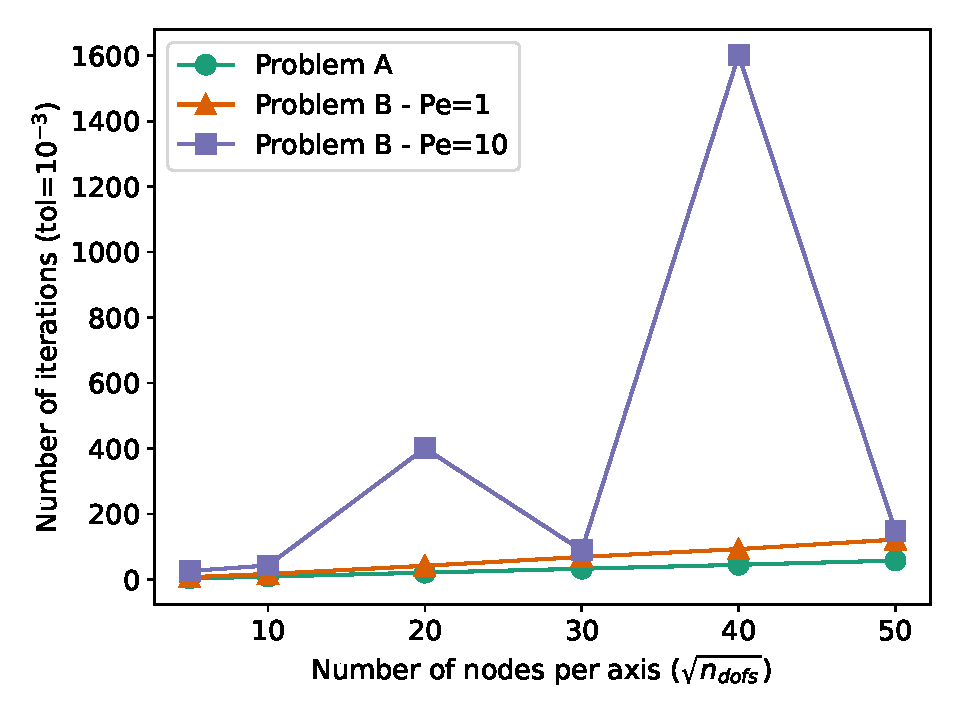
\includegraphics[width=0.95\linewidth]{images/cg_its}
\end{frame}

\subsection{GMRES}

\begin{frame}[fragile]{\textbf{4. GMRES}}
	The Generalized Minimal RESidual method (GMRES) is a projection method that aims a minimizing the residual norm over all the vectors of the Krylov subspace that is being built ($x^{(0)}+\mathcal{K}^{(m)}$).
	
	
	The GMRES algorithm uses the Arnoldi iteration for numerical stability. The Arnoldi iteration
	produces $\mathcal{H}^{(n)}$, an $(n + 1) \times n$ upper Hessenberg matrix, and $\mathcal{Q}^{(n)}$, a matrix whose columns make up an	orthonormal basis of $\mathcal{K}^{(n)}(\mathcal{A}, b)$, such that $\mathcal{A}\mathcal{Q}^{(n)} = \mathcal{Q}^{(n+1)}\mathcal{H}^{(n)}$. The GMRES algorithm finds the vector	$x^{(n)}$ that minimizes the norm $\lVert (\mathcal{A},x^{(n)}) - b \rVert$ where $x^{(n)} = (\mathcal{Q}^{(n)},y^{(n)}) + x^{(0)}$ for some $y^{(n)} \in \mathbb{R}$
	
	 The algorithm is quite complex. I  give it here, but you will need to take a dive into the code to acquire a better understanding of it.


	
\end{frame}

\begin{frame}[fragile]{\textbf{4. GMRES Algorithm}}

\begin{algorithm}[H]
	\KwIn{A matrix $\mathcal{A}$, a RHS $b$, an initial guess $x^{(0)}$, a maximum number of Krylov vectors $p$ and a tolerance $\mathrm{tol}$}

	$\mathcal{Q}\leftarrow$empty(size($b$),$p+1$)
	
	$\mathcal{H}\leftarrow$empty($p+1$,$p$)
	
	$e_1 \leftarrow$ empty(size($b$),$p+1$) $ + [1,\dots,0]^T$
	
	$r^{(0)} = b-\mathcal{A}x^{(0)}$
	
	$\beta = \lVert r^{(0)} \rVert$

	
	$\mathcal{Q}_{:,0} = \frac{r^{(0)}}{\lVert r^{(0)} \rVert}$
	
	

	\For{$j=0 \dots p-1$}
	{
	   $\mathcal{Q}_{:,j+1} \leftarrow (\mathcal{A},\mathcal{Q}_{:,j})$
	   
	   \For{$i=0 \dots j$}{
	   	  $\mathcal{H}_{i,j} = (\mathcal{Q}^{T}_{:,i},\mathcal{Q}_{:,j+1})$
	   	   
	   	   $\mathcal{Q}_{:,j+1} \leftarrow  \mathcal{Q}_{:,j+1} - (\mathcal{A},\mathcal{Q}_{:,j})$
	   }
	   
	   $\mathcal{H}_{j+1,j} = \lVert \mathcal{Q}^{(j)} \rVert$
	   

	  
	  solve the least-square problem: $\mathcal{H}_{:j+2,:j+1}^{T} \mathcal{H}_{:j+2,:j+1} y = \beta \mathcal{H}_{:j+2,:j+1}^{T}  e_1$
	
	  $x^{j+1} = x^{(0)} + \mathcal{Q}_{:,:j+1}$ y
	  
	  \If {$\lVert r^{(j+1)} \rVert < \mathrm{tol}$}
	  {
	  	\textbf{break}
	  }
	}
\end{algorithm}

\end{frame}

\begin{frame}
	\frametitle{\textbf{4. GMRES results}}
	\centering
	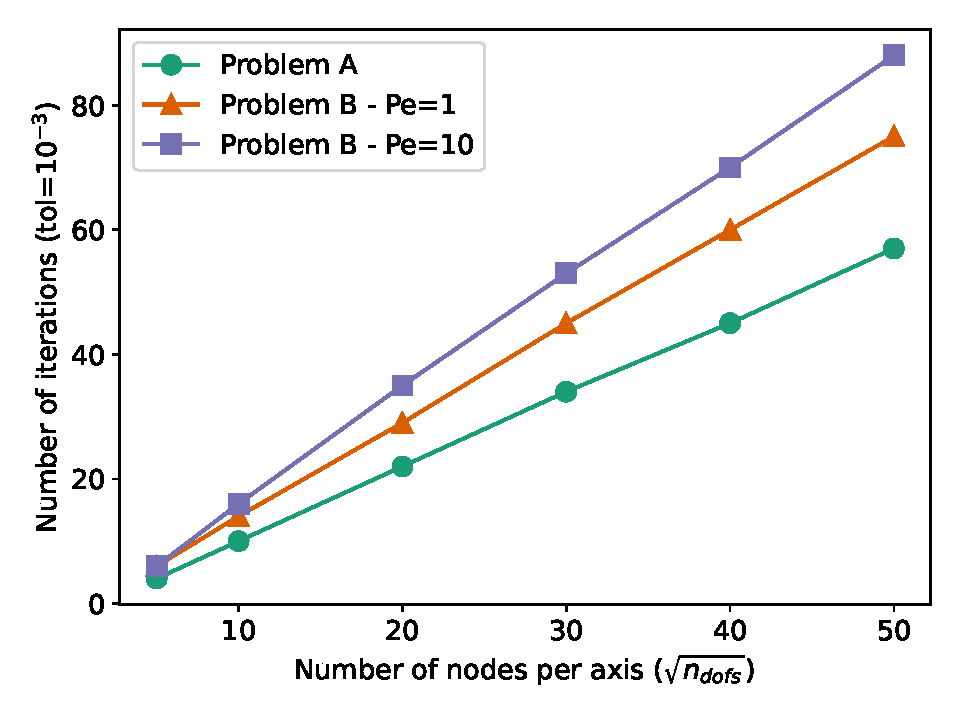
\includegraphics[width=0.95\linewidth]{images/gmres_its}
\end{frame}



    	

    
	\section{Final remarks}
    \begin{frame}
	\frametitle{\textbf{6. Final remarks}}

 
    
\end{frame}
	\begin{frame}
	\frametitle{\textbf{5. Conclusions}}

        
\end{frame}
	
	\nocite{*} %If I want all references in the .bib file to appear even without citation
	\begin{frame}[allowframebreaks, noframenumbering]
	\frametitle{\textbf{References}}
    \bibliographystyle{ieeetr}
    \footnotesize
    \bibliography{references.bib}

	
\end{frame}    

	%Additional slides
    \appendix
    % \include{frames/additional_slide}

\end{document}